%\documentclass[prd,nofootinbib]{revtex4}
%\documentclass[10pt]{article}
\documentclass[10pt]{NSF}

\usepackage{latexsym}
%\usepackage[top=1in, bottom=1in, left=1in, right=1in]{geometry}
\usepackage{amsfonts}
\usepackage{amsmath}
\usepackage{amssymb}
\usepackage{upgreek}
\usepackage{bm}
\usepackage{dsfont}
\usepackage{dcolumn}
\usepackage{epsfig}
\usepackage{graphicx}
\usepackage{graphics}
\usepackage{placeins}
\usepackage{subfigure}

% begin equation, itemize, etc.

\def\be{\begin{equation}}
\def\ee{\end{equation}}
\def\bi{\begin{itemize}}
\def\ei{\end{itemize}}
\def\ben{\begin{enumerate}}
\def\een{\end{enumerate}}
\def\i{\item{}}
\newcommand{\bs}[1]{\boldsymbol{#1}}
\newcommand{\mb}[1]{\mathbf{#1}}

\begin{document}

%%%%%%%%%%%%%%%%%%%%%%%%%%%%%%%%%%%%%%%%%%%%%%%%%%%%%%%%%%%%%%%%%%%%%%
\title{Simulating a PTA with metronomes and microphones:\\
A user's guide for a double-metronome timing \& correlation 
demonstration}
\maketitle
\tableofcontents

%%%%%%%%%%%%%%%%%%%%%%%%%%%%%%%%%%%%%%%%%%%%%%%%%%%%%%%%%%%%%%%%%%%%%%
\newpage
\subsection{Purpose}
\label{s:purpose}

The purpose of the double-metronome timing and correlation 
demonstration is to illustrate (using two metronomes and a 
microphone) how a pulsar timing array (PTA) uses correlation
methods to search for gravitational-wave signals in pulsar
timing data.
As a gravitational wave transits the line-of-sight between 
the Earth and an array of pulsars in our galaxy, it 
induces correlations in the measured timing residuals across 
pairs of pulsars in the array.
In this demonstration, radio pulses from an array of pulsars
are represented by ticks of an array of metronomes
(only two metronomes are needed for this demo);
radio receivers on Earth are represented by a single microphone;
and the passage of a gravitational wave is represented by the 
motion of the microphone
(basically, the ``Earth-term" in pulsar timing language).
The motion of the microphone Doppler shifts the received 
frequency of the metronome pulses, changing the arrival times of 
these pulses at the microphone from that in the absence
of microphone motion.

This demonstration is best suited for undergraduates or 
senior-level highschool students.
It illustrates the following techniques used in pulsar 
timing analyses:
\ben
\i Estimate the pulse period and calculate a reference 
pulse profile (i.e., a template) by folding data consisting 
of several pulses.

\i Estimate the times of arrival (TOAs) of the pulses by
correlating the template pulse profile with the data.

\i Calculate the timing residuals by subtracting the 
expected TOAs (assuming a simple timing model) from 
actual TOAs, which were estimated in the previous step.

\i Improve the estimate of the pulse period by removing a
linear trend from the timing residuals.

\i Show that the timing residuals for a pair of pulsars are
correlated as a function of the angular seperation between the
lines-of-sights to the two pulsars.

\een
%
For less-mathematically-inclined audiences, the mathematical 
description of
the demonstration will need to be reduced accordingly.
But the visual representation of the residuals from the two 
metronomes being shifted in phase relative to one another
by an amount equal to their angular separation should be 
comprehensible to all audiences.

%%%%%%%%%%%%%%%%%%%%%%%%%%%%%%%%%%%%%%%%%%%%%%%%%%%%%%%
\subsection{Required hardware}
\label{s:hardware}

Two metronomes are required, 
Seiko model SQ50-V quartz 
metronome being the prefered choice.
This model has adjustable beats-per-minute (bpm) up 
to 208 bpm, adjustable volume, and 
two different tempo sounds (mode $a$ and mode $b$,
with mode $b$ having a slightly higher pitch).
Having two modes is helpful in distinguishing the
pulses from the individual metronomes, since the 
pulse profiles are different.

One also needs some type of microphone, either an 
external USB microphone or an internal microphone,
connected to a laptop that is 
set up to run the relevant data analysis routines
(see Secs.~\ref{s:software}, \ref{s:PTAdemo0GUI}, \ref{s:PTAdemo2GUI} for details).
I have found that the internal microphone on my laptop 
works best since it has ambient noise reduction,
although it is somewhat incovenient (awkward) to 
physically move the laptop to 
simulate the passage of a gravitational wave.
To produce uniform circular motion of the microphone, 
one can either swing an external USB microphone 
in a circle supporting
it by its cable, or place the laptop on a rotating platform 
that can turn freely.

Michele Vallisneri suggested doing this demo using
three cellphones: two acting as pulsars by running 
metronome apps, and the other acting as the radio 
receivers on Earth, behaving as a microphone and 
running a javascript implementation of the data analysis
routines.

In addition, one needs an open space covering an area of 
about $10~{\rm ft}\times 5~{\rm ft}$ 
for the placement of the two metronomes and microphone.
As schematic diagram of the setup is shown in
Figure~\ref{f:setup}.
A photograph of an actual real-world setup used to take the
data described in this user's guide is shown in
Figure~\ref{f:actualsetup}.
%
\begin{figure*}[hbtp!]
\begin{center}
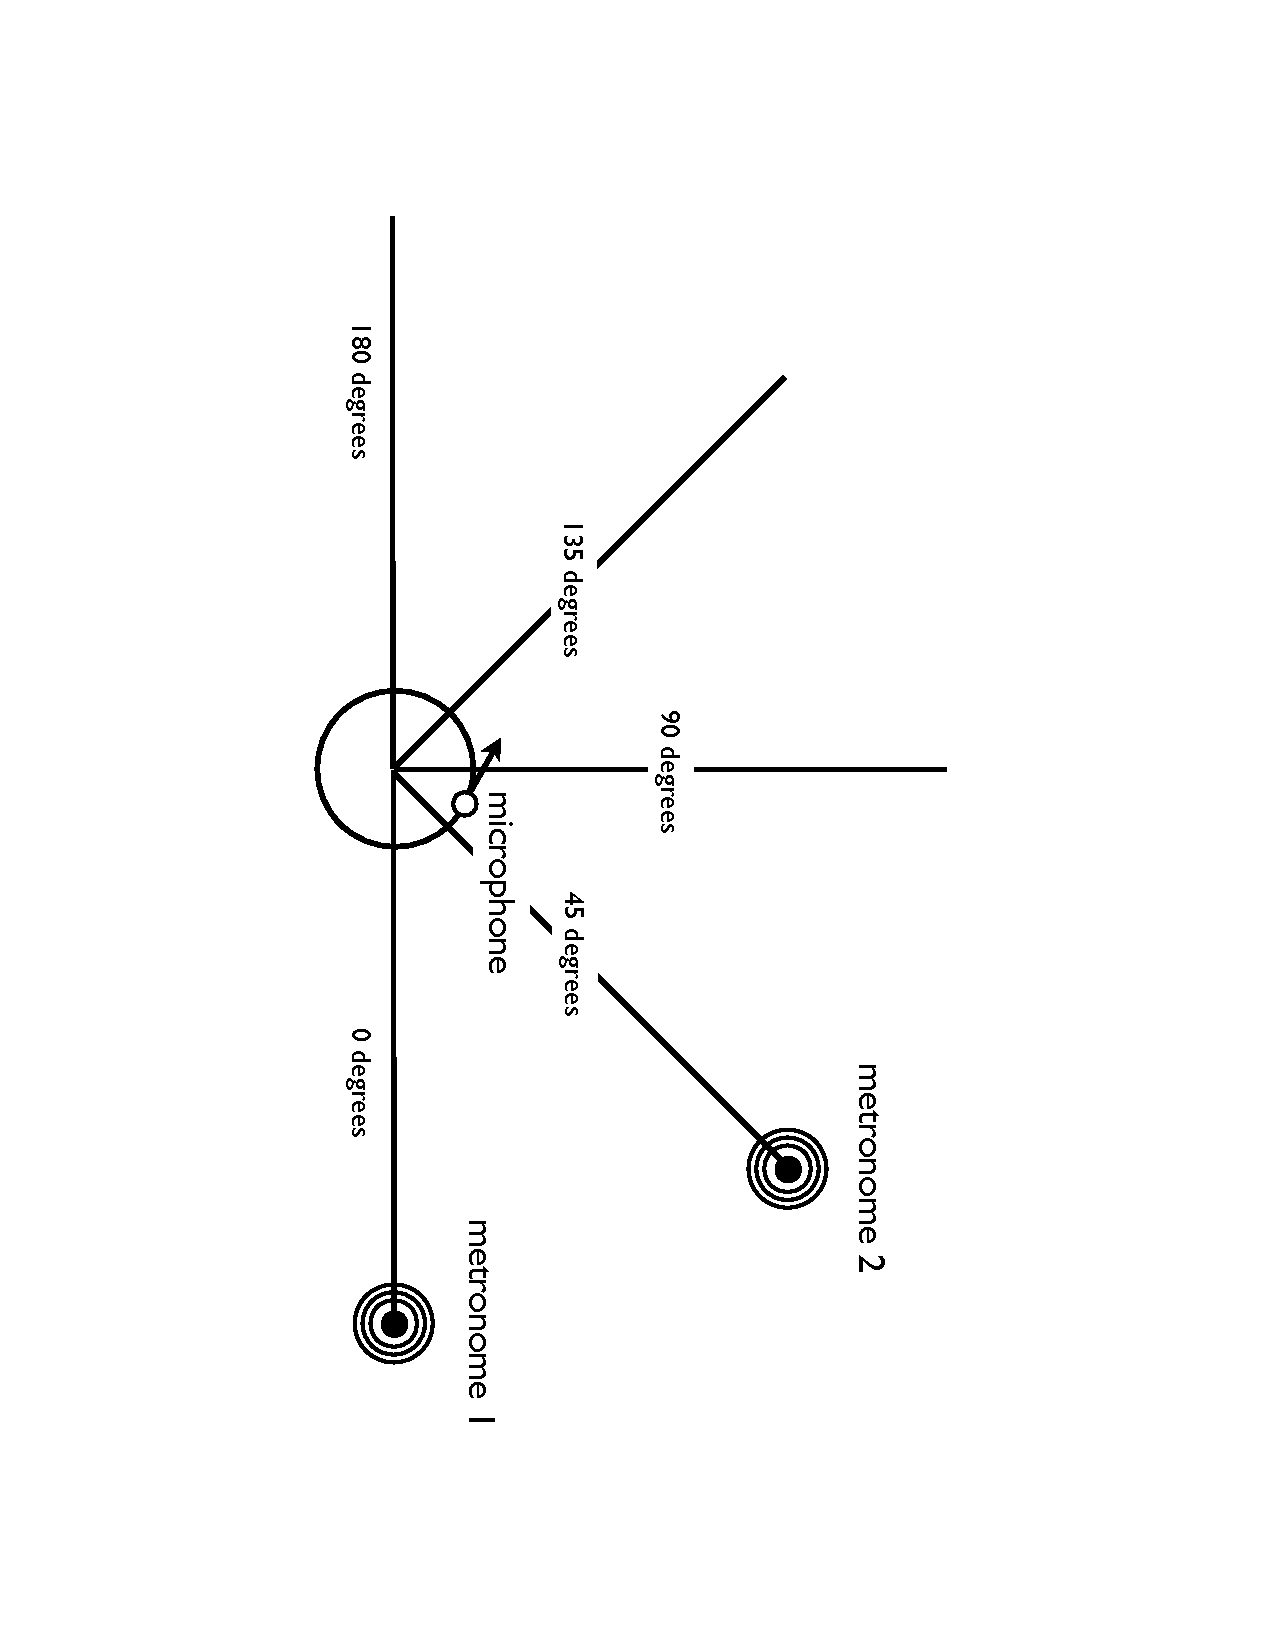
\includegraphics[clip=true, angle=90, width=\textwidth]{figures/setup-circular}
\caption{Schematic diagram showing the location of the microphone 
and metronomes for the different analyses.
The stationary microphone is located at the origin;
the moving microphone undergoes uniform circular motion, 
indicated by the counter-clockwise circle.
Metronome 2 is placed at angular location $45^\circ$ in this figure,
but will be placed at the other angular locations for different parts
of this demo.}
\label{f:setup}
\end{center}
\end{figure*}
%
\begin{figure*}[hbtp!]
\begin{center}
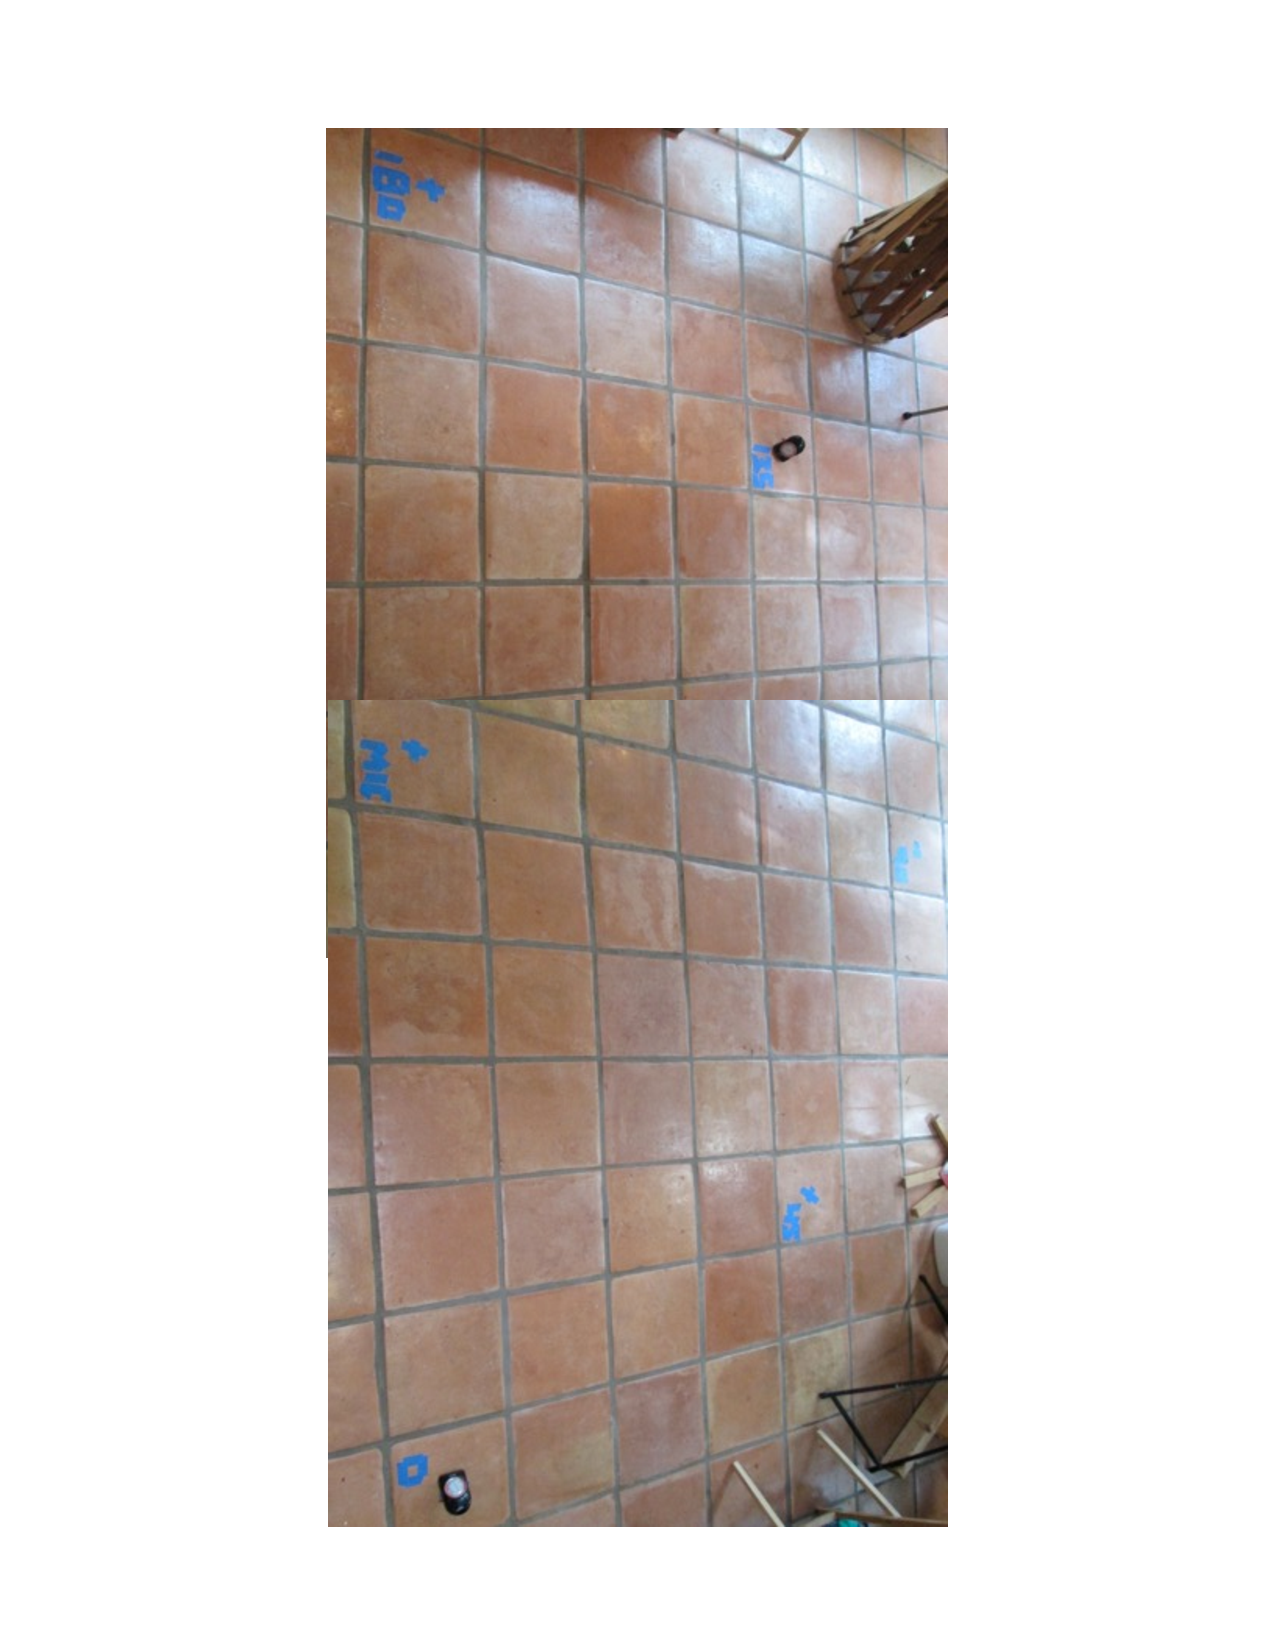
\includegraphics[clip=true, angle=90, width=\textwidth]{figures/actualsetup}
\caption{Photograph of an actual setup for data taking.
Metronome 1 is shown at angular location $0^\circ$; 
metronome 2 at angular location $135^\circ$.
The separation between the microphone (located at the origin) and the
metronomes at the edge of a semi-circle is approximately 5~feet.}
\label{f:actualsetup}
\end{center}
\end{figure*}

%%%%%%%%%%%%%%%%%%%%%%%%%%%%%%%%%%%%%%%%%%%%%%%%%%%%%%%%%%%%
\subsection{Required software}
\label{s:software}

Both Matlab and Python-based routines exist for doing
the data analysis.
These includes: 
(i) audio recording and play back of metronome pulses, 
(ii) data folding, 
(iii) pulse profile calculation,
(iv) matched-filtering estimation of pulse arrival times, 
(v) timing residual calculation, 
(vi) linear detrending of timing residuals, 
(vii) fitting of sinusoids to the timing residuals, and 
(viii) correlation coefficient calculation.
Two Python-based GUIs exist for performing the two main
data taking and data analysis tasks:  
{\tt PTAdemo0GUI.py} (for 
analyzing the single-metronome pulse data) and
{\tt PTAdemo2GUI.py} 
(for analyzing the double-metronome pulse data).
These two GUIs and some of the underlying routines 
are described in detail in the following sections.

%%%%%%%%%%%%%%%%%%%%%%%%%%%%%%%%%%%%%%%%%%%%%%%%%%%
\subsection{Single-metronome pulse analysis}
\label{s:PTAdemo0GUI}

\subsubsection{The GUI: {\tt PTAdemo0GUI.py}}

A screenshot of {\tt PTAdemo0GUI.py} is shown in 
Figure~\ref{f:PTAdemo0GUI}.
The GUI has space for plots of:
(i) pulses from the individual metronomes,
(ii) pulse profiles (obtained by folding the pulse data),
and 
(iii) timing residuals.
The GUI also has several text entry fields and buttons, whose functions
are described below:
%
\begin{figure*}[hbtp!]
\begin{center}
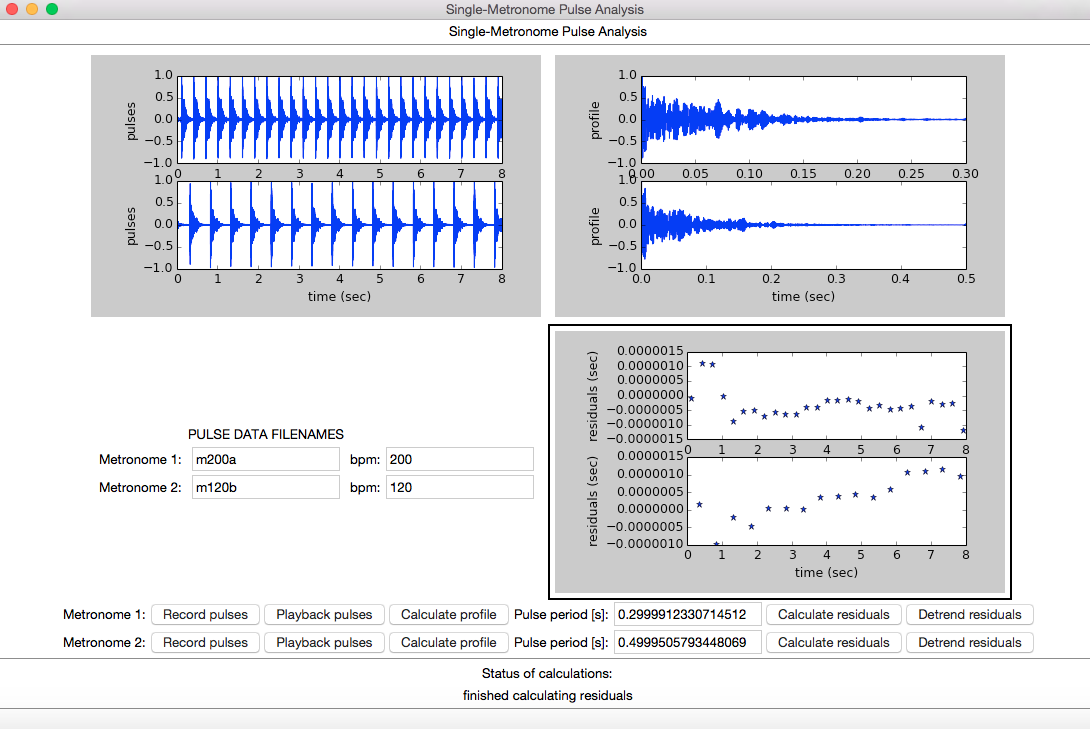
\includegraphics[clip=true, angle=0, width=\textwidth]{figures/PTAdemo0GUI.png}
\caption{Python GUI for the single-metronome pulse analysis.}
\label{f:PTAdemo0GUI}
\end{center}
\end{figure*}

{\bf Record pulses}:
Records audio pulse data from a metronome, and save the corresponding
timeseries to an ascii {\tt .txt} file with file prefix specified by 
the 'PULSE DATA FILENAMES' text entry boxes (default {\tt m200a} or {\tt m120b}).
The 'bpm' text entry boxes have the beats-per-minute settings for 
the two metronomes. 
The pulse recording routine is hard-coded to record 6~seconds of data.

{\bf Playback pulses}:
Plays back and plots the audio pulse data saved in
{\tt m200a.txt} or {\tt m120b.txt}.

{\bf Calculate\ profile}:
Either 
(i) calculates the pulse period $T_p$ and pulse profile directly 
by folding the metronome data,
and then saves the profile to the file 
{\tt m200a\_profile.txt} or {\tt m120b\_profile.txt}, or 
(ii) reads in the pulse profile data that has already been saved 
in these files.
Method (i) is used only the first time the analysis is run.
If the pulse profiles are read-in from the files 
{\tt m200a\_profile.txt} and {\tt m120b\_profile.txt}, the text entry 
boxes for the pulse periods need to be entered by hand.
For both cases, the pulse profile is plotted from 0 to $T_p$.

{\bf Calculate residuals}:
Calculates the timing residuals by subtracting the expected 
TOAs from the measured TOAs of the pulses:
%
\be
%\delta t_{Ii} = \tau^{\rm meas}_{Ii} - \tau^{\rm exp}_{Ii} 
{\rm residual}(i) = {\rm measured}(i) - {\rm expected}(i)
\ee
%
The expected arrival times are defined by a simple timing model
%
\be
%\tau^{\rm exp}_{Ii} = \tau^{\rm meas}_{I1} + (i-1)T_I
{\rm expected}(i) = {\rm measured}(i_0) + (i-i_0)T_p
\ee
%
which is just the measured TOA of the pulse having the 
largest correlation (see below) plus 
integer multiples of the pulse period $T_p$ of the metronome.
The measured TOAs are obtained by correlating time-shifted 
pulse profiles with the data.
Mathematically, the correlation function is defined by
%
\be
C_I(t) ={\cal N}_I
\int_0^{f_{\rm Nyq}} df\> 
e^{i2\pi ft}\tilde y(f) \tilde p_I^*(f)\,,
\qquad
{\cal N}_I
=\left[\int_0^{f_{\rm Nyq}} df\> 
|\tilde p_I^*(f)|^2\right]^{-1}
\ee
%
where $\tilde y(f)$ is the Fourier transform of the
measured pulse data $y(t)$, and $\tilde p_I(f)$ is the
Fourier transform of the template pulse profiles
$p_I(t)$ for the two metronomes, $I=1,2$.
$C_I(t)$ will have local maxima at the arrival 
times of the pulses.
The normalization constant ${\cal N}_I$ is included  
so that the values of the correlation function at the 
estimated arrival times are estimates of the amplitudes
of the pulses.

{\bf Detrend residuals}:
Improves the estimate of the pulse period for 
a metronome by removing a linear trend 
from the timing residuals, if such a trend exists.
Detrending may change the estimate of the pulse period
by 1-2 microseconds.
The updated period is displayed in the `Pulse period'
text entry box.

\subsubsection{Steps for doing the analysis}

\ben

\i Record pulses from each metronome separately, keeping the 
microphone stationary.
The microphone should be located at the origin of coordinates and the two
metronomes should be at angular location $0^\circ$.
The file prefixes and bpms in the text entry boxes should be chosen
to match the physical settings of the metronome.

\i After recording the pulse data for each metronome, you can play it 
back, calculate the corresponding pulse profile and period, calculate
the residuals, and detrend the residuals, by simply pressing the relevant
GUI buttons.
\een

This analysis produces two pulse profile data files 
(e.g., {\tt m200a\_profile.txt} and {\tt m120b\_profile.txt}) and the 
associated pulse periods $T_1$, $T_2$, which are needed for the 
double-metronome pulse analysis described in the next section.

%%%%%%%%%%%%%%%%%%%%%%%%%%%%%%%%%%%%%%%%%%%%%%%%%%%
\subsection{Double-metronome pulse analysis}
\label{s:PTAdemo2GUI}

\subsubsection{The GUI: {\tt PTAdemo2GUI.py}}

A screenshot of {\tt PTAdemo2GUI.py} is shown in 
Figure~\ref{f:PTAdemo2GUI}.
The GUI has space for plots of:
(i) pulses from the two metronomes running simultaneously,
(ii) reference pulse profiles for the two metronomes, which were 
calculated using {\tt PTAdemo0GUI.py}, and
(iii) timing residuals for the two metronomes.
The GUI also has several text entry fields and buttons, whose functions
are described below:
%
\begin{figure*}[hbtp!]
\begin{center}
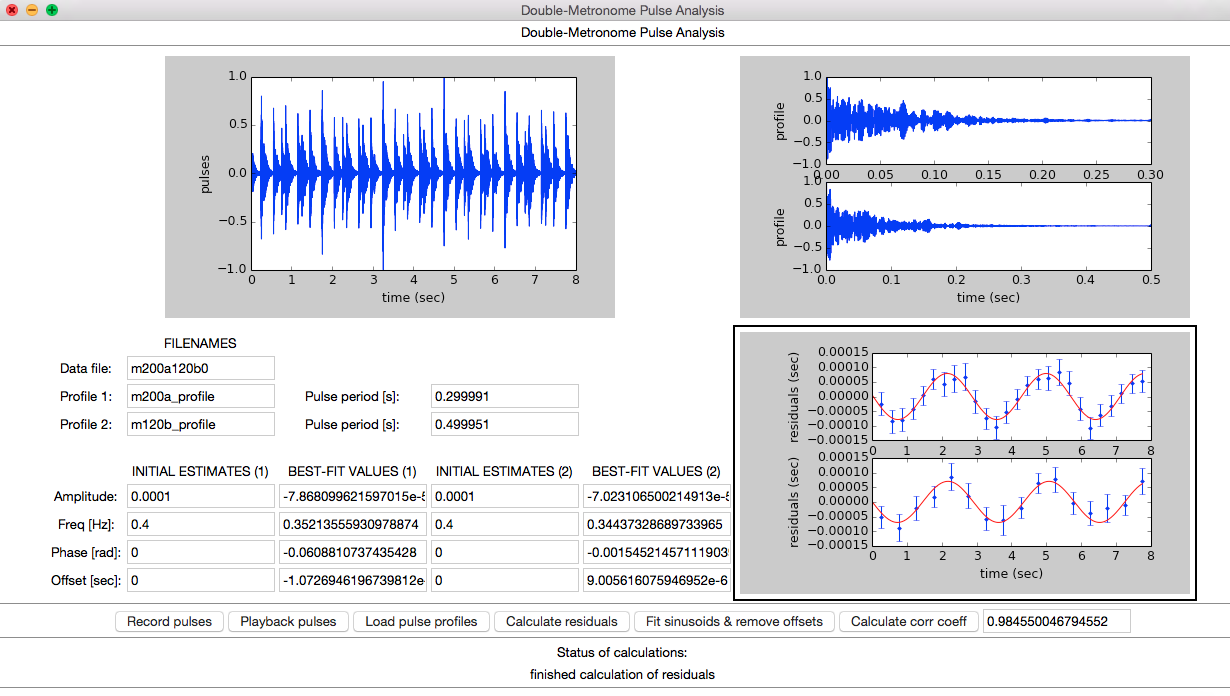
\includegraphics[clip=true, angle=0, width=\textwidth]{figures/PTAdemo2GUI.png}
\caption{Python GUI for the double-metronome pulse analysis.}
\label{f:PTAdemo2GUI}
\end{center}
\end{figure*}

{\bf Record pulses}:
Records audio pulse data from the two metronomes running simultaneously, 
and then saves the corresponding timeseries to an ascii {\tt .txt} file 
with file prefix specified by the `Data file' text entry box under 
the 'FILENAMES' label (default {\tt m200a120b0}).

{\bf Playback pulses}:
Plays back and plots the audio pulse data saved in
{\tt m200a120b0.txt}.

{\bf Load pulse profiles}:
Reads-in and plots the reference pulse profiles for the two 
metronomes, which were calculated by {\tt PTAdemo0GUI.py} and
were saved in ascii {\tt .txt} files specified by 
the 'Profile 1,2' text entry boxes under the `FILENAMES' label
(default {\tt m200a\_profile.txt} and {\tt m120b\_profile}).
The text entry boxes for the pulse periods should be filled with 
in with the values calculated by {\tt PTAdemo0GUI.py}.

{\bf Calculate residuals}:
Calculates the timing residuals as described previously
for {\tt PTAdemo0GUI.py}.

{\bf Fit sinusoids \& remove offsets}:
Simultaneously removes constant offsets and calculates best-fit 
sinusoids to the timing residuals for the two metronomes, using 
initial estimates for the amplitude, frequency, and phase of
the sinusoids, and the constant offset given in the text entry boxes labeled 
'INITIAL ESTIMATES (1,2)' (defaults $1\times 10^{-4}$, $0.5~{\rm Hz}$,
0~radians, and 0~sec).
The constant offset arises from the arbitrariness of setting the 
timing residual of the pulse with the highest correlation to zero.
The best-fit parameter values calculated by 'Fit sinusoids \& remove offsets' 
are written to the text entry boxes labeled `BEST-FIT VALUES (1,2)'.

{\bf Calculate corr coeff}:
Calculates the time-averaged correlation coefficient between 
the best-fit sinusoids for the two sets of timing residuals.
If we denote the best-fit sinusoids by $x(t)$ and $y(t)$, then
%
\be
{\rm corr\ coeff}\equiv 
\frac{\langle xy\rangle}{\sqrt{\langle x^2\rangle \langle y^2\rangle}}
\,,
\quad{\rm where}\quad
\langle x y\rangle \equiv \frac{1}{T}\int_0^T dt\> x(t)y(t)
\ee
%
Theoretically, the value of the correlation coefficient 
should equally $\cos\chi$, where $\chi$ is the separation angle 
between the line-of-sights to the
two metronomes as described in Section~\ref{s:discussion}.

\subsubsection{Steps for doing the analysis}

\ben

\i Start by placing both metronomes at the same angular location $0^\circ$
and at the same distance $L\sim 1~{\rm m}$ from the origin.
With both metronomes running simultaneously, record the audio data
while setting the microphone in uniform circular motion 
about the origin:
%
\be
\vec r(t) 
= A\left[\cos(2\pi f_0 t + \phi_0)\, \hat x + \sin(2\pi f_0 t+\phi_0)\, \hat y\right]
\label{e:UCM}
\ee
%
Typically, it is best to have 
$A\approx 10~{\rm cm}$ (=0.1~m) and period of oscillation 
$T_0\equiv 1/f_0\approx 2~{\rm s}$.
This leads to microphone-induced timing residuals of order 
$A/c\approx 3\times 10^{-4}~{\rm s}$, where 
$c=340~{\rm m/s}$ is the
speed of sound in air.
(See Section~\ref{s:discussion} for a detailed discussion
of microphone-induced timing residuals.)
This turns out to be more than an order-of-magnitude larger than
the precision to which we can estimate the TOAs
of the metronome pulses, meaning that we can easily observe the
effect of microphone motion in the timing-residual data.

\i After recording the double-metronome data, you can play it back, 
load the pulse profiles, and calculate and detrend the residuals 
for each metronome.
The timing residuals induced by the microphone motion should be
sinusoidal and have large signal-to-noise ratio.
You should then fit sinusoids to the residuals for each metronome, 
adjusting the 'INITIAL GUESS' amplitudes, frequencies, and phases if 
necessary.  
(The initial guesses just have to be close, not exact.)
Finally, you should calculate the correlation coefficient, 
which should have a value very close to 1 for this case, since 
the two microphones are at the same angular location.

\i Repeat the above two steps but with metronome 2 at different
angular locations ($45^\circ$, $90^\circ$, $135^\circ$, and $180^\circ$)
with respect to metronome 1 (which should always remain at $0^\circ$).
The motion of the microphone should be as similar as possible to that
for Step 1.
Change the name of the file prefix in the 
`Data file' text entry box to {\tt m200a120bXX}, 
where {\tt XX} is {\tt 45}, {\tt 90}, {\tt 135}, and {\tt 180}, 
to reflect the change in the angular
location of metronome 2.
You should find that the correlation coefficient is approximately
equal to $\cos\chi$, where $\chi=45^\circ$, $90^\circ$, $135^\circ$ and $180^\circ$
is the angular separation of the two metronomes.

\een

This analysis produces data files ({\tt m200a120bXX.txt}, 
where {\tt XX} is {\tt 0}, {\tt 45}, {\tt 90}, {\tt 135}, and {\tt 180}),
containing the double-metronome pulse timeseries.

%%%%%%%%%%%%%%%%%%%%%%%%%%%%%%%%%%%%%%%%%%%%%%%%%%%%%%%
\subsection{Discussion}
\label{s:discussion}

\subsubsection{Microphone-induced timing residuals}
\label{s:timingresiduals}

Theoretically, the timing residuals for metronome $I=1,2$ induced 
by a moving microphone are given by
%
\be
%\delta t_I^{\rm mic}(t)
{\rm residual}_I(t)
\equiv\frac{\Delta L_I(t)}{c}
=\frac{L_I(t)-L_I}{c}
\simeq 
-\frac{1}{c} \hat u_I\cdot \vec r(t)
\label{e:timingresidual}
\ee
%
where $L_I(t)$ is the distance between 
metronome $I$ and the location of the 
microphone $\vec r(t)$ at time $t$,
and $L_I$ is the nominal distance between the
metronome and the microphone.
This is just the change in the 
metronome pulse-propagation time due to the motion
of the microphone relative to metronome $I$.
The last (approximate) equality above is valid 
if we ignore 
correction terms of order $A/L_I\sim 0.1$, where 
$A\approx 5~{\rm cm}$ is the amplitude of the 
microphone motion and $L_I\approx 1~{\rm m}$ 
is the distance from the metronome to the 
microphone when it is at the origin.
These correction terms arise from the finite distance
of the metronome from the microphone; in other words,
the pulse wavefronts are actually curved not planar.
Including the next-order correction term gives us
%
\be
{\rm residual}_I(t)
\simeq 
-\frac{1}{c}
\left[\hat u_I\cdot \vec r(t)+\frac{1}{2L_I}
\left((\hat u_I\cdot \vec r(t))^2 - |\vec r(t)|^2\right)\right]
\ee
%

For the microphone undergoing uniform circular motion (\ref{e:UCM}):
%
\be
%\delta t_I^{\rm mic}(t) 
{\rm residual}_I(t)
\simeq -\frac{A}{c}\cos(2\pi f_0 t+\phi_0-\zeta_I)
%+\frac{A}{c}\frac{A}{L}\sin^2(2\pi f_0 t + \phi_0 - \zeta_I)+ {\cal O}\left((A/L)^2\right)
\ee
%
%
where $\zeta_I$ is the angle that the location of metronome 
makes with respect to the $x$-axis, and where we have ignored
the higher-order correction terms to the residual.
Using the trig indentity 
%
\be
\cos A\cos B =\frac{1}{2}\left[
\cos(A+B) + \cos(A-B)
\right]
\ee
%
it is fairly easy to show that the time-averaged 
correlation coefficient of
the microphone-induced timing residuals for metronomes 1 and 2 is
%
\be
{\rm corr\ coeff} \simeq \cos\chi
\ee
%
where $\chi\equiv \zeta_1-\zeta_2$ is the angle between the line-of-sights
to the two metronomes.
This equality is correct to order $(A/L)^2$.
(Since the timing residuals 
%$\delta t_1^{\rm mic}(t)$ and $\delta t_2^{\rm mic}(t)$
for the two metronomes
are evaluated at different times, we actually correlate the 
best-fit sinusoids to the timing residuals.)
This dependence of the correlation coefficient on the angle
between the two metronomes is confirmed (roughly) by the 
double-metronome analysis.

%%%%%%%%%%%%%%%%%%%%%%%%%%%%%
\subsubsection{Technical remarks about uniform circular motion}

We have chosen uniform circular motion for the microphone
and not (linear) sinusoidal motion in a plane, since the angular
dependence of the correlation coefficient for linear motion 
would depend not only on the angular separation $\chi$ of the two 
metronomes, but also on their angular separation with respect to
the plane of oscillation of the microphone.
In addition, any linear sinusoidal motion can be written as a 
superposition of counter-clockwise and clockwise uniform circular
motions.
In fact, {\em any} motion whatsoever can be written as a linear superposition
of sinusoidal motions having different frequencies and planes of
oscillations, as a consequence of Fourier's theorem.
Thus, there is no loss in generality in considering the simple
uniform circular motion case.

Finally, we note that the effect of uniform circular motion on the 
timing residuals 
is exactly what one sees in real pulsar-timing timing residuals if the 
yearly orbital motion 
of the Earth around the Sun is not taken into account in the timing
model for the pulsars.

\end{document}
